% Options for packages loaded elsewhere
\PassOptionsToPackage{unicode}{hyperref}
\PassOptionsToPackage{hyphens}{url}
%
\documentclass[
  english,
  man]{apa6}
\usepackage{amsmath,amssymb}
\usepackage{lmodern}
\usepackage{ifxetex,ifluatex}
\ifnum 0\ifxetex 1\fi\ifluatex 1\fi=0 % if pdftex
  \usepackage[T1]{fontenc}
  \usepackage[utf8]{inputenc}
  \usepackage{textcomp} % provide euro and other symbols
\else % if luatex or xetex
  \usepackage{unicode-math}
  \defaultfontfeatures{Scale=MatchLowercase}
  \defaultfontfeatures[\rmfamily]{Ligatures=TeX,Scale=1}
\fi
% Use upquote if available, for straight quotes in verbatim environments
\IfFileExists{upquote.sty}{\usepackage{upquote}}{}
\IfFileExists{microtype.sty}{% use microtype if available
  \usepackage[]{microtype}
  \UseMicrotypeSet[protrusion]{basicmath} % disable protrusion for tt fonts
}{}
\makeatletter
\@ifundefined{KOMAClassName}{% if non-KOMA class
  \IfFileExists{parskip.sty}{%
    \usepackage{parskip}
  }{% else
    \setlength{\parindent}{0pt}
    \setlength{\parskip}{6pt plus 2pt minus 1pt}}
}{% if KOMA class
  \KOMAoptions{parskip=half}}
\makeatother
\usepackage{xcolor}
\IfFileExists{xurl.sty}{\usepackage{xurl}}{} % add URL line breaks if available
\IfFileExists{bookmark.sty}{\usepackage{bookmark}}{\usepackage{hyperref}}
\hypersetup{
  pdftitle={Item Characteristic Curves generated from common CTT Item Statistics},
  pdfauthor={Diego Figueiras1 \& John T. Kulas1},
  pdflang={en-EN},
  pdfkeywords={keywords},
  hidelinks,
  pdfcreator={LaTeX via pandoc}}
\urlstyle{same} % disable monospaced font for URLs
\usepackage{graphicx}
\makeatletter
\def\maxwidth{\ifdim\Gin@nat@width>\linewidth\linewidth\else\Gin@nat@width\fi}
\def\maxheight{\ifdim\Gin@nat@height>\textheight\textheight\else\Gin@nat@height\fi}
\makeatother
% Scale images if necessary, so that they will not overflow the page
% margins by default, and it is still possible to overwrite the defaults
% using explicit options in \includegraphics[width, height, ...]{}
\setkeys{Gin}{width=\maxwidth,height=\maxheight,keepaspectratio}
% Set default figure placement to htbp
\makeatletter
\def\fps@figure{htbp}
\makeatother
\setlength{\emergencystretch}{3em} % prevent overfull lines
\providecommand{\tightlist}{%
  \setlength{\itemsep}{0pt}\setlength{\parskip}{0pt}}
\setcounter{secnumdepth}{-\maxdimen} % remove section numbering
% Make \paragraph and \subparagraph free-standing
\ifx\paragraph\undefined\else
  \let\oldparagraph\paragraph
  \renewcommand{\paragraph}[1]{\oldparagraph{#1}\mbox{}}
\fi
\ifx\subparagraph\undefined\else
  \let\oldsubparagraph\subparagraph
  \renewcommand{\subparagraph}[1]{\oldsubparagraph{#1}\mbox{}}
\fi
% Manuscript styling
\usepackage{upgreek}
\captionsetup{font=singlespacing,justification=justified}

% Table formatting
\usepackage{longtable}
\usepackage{lscape}
% \usepackage[counterclockwise]{rotating}   % Landscape page setup for large tables
\usepackage{multirow}		% Table styling
\usepackage{tabularx}		% Control Column width
\usepackage[flushleft]{threeparttable}	% Allows for three part tables with a specified notes section
\usepackage{threeparttablex}            % Lets threeparttable work with longtable

% Create new environments so endfloat can handle them
% \newenvironment{ltable}
%   {\begin{landscape}\centering\begin{threeparttable}}
%   {\end{threeparttable}\end{landscape}}
\newenvironment{lltable}{\begin{landscape}\centering\begin{ThreePartTable}}{\end{ThreePartTable}\end{landscape}}

% Enables adjusting longtable caption width to table width
% Solution found at http://golatex.de/longtable-mit-caption-so-breit-wie-die-tabelle-t15767.html
\makeatletter
\newcommand\LastLTentrywidth{1em}
\newlength\longtablewidth
\setlength{\longtablewidth}{1in}
\newcommand{\getlongtablewidth}{\begingroup \ifcsname LT@\roman{LT@tables}\endcsname \global\longtablewidth=0pt \renewcommand{\LT@entry}[2]{\global\advance\longtablewidth by ##2\relax\gdef\LastLTentrywidth{##2}}\@nameuse{LT@\roman{LT@tables}} \fi \endgroup}

% \setlength{\parindent}{0.5in}
% \setlength{\parskip}{0pt plus 0pt minus 0pt}

% \usepackage{etoolbox}
\makeatletter
\patchcmd{\HyOrg@maketitle}
  {\section{\normalfont\normalsize\abstractname}}
  {\section*{\normalfont\normalsize\abstractname}}
  {}{\typeout{Failed to patch abstract.}}
\patchcmd{\HyOrg@maketitle}
  {\section{\protect\normalfont{\@title}}}
  {\section*{\protect\normalfont{\@title}}}
  {}{\typeout{Failed to patch title.}}
\makeatother
\shorttitle{CTT ICCs}
\keywords{keywords\newline\indent Word count: X}
\DeclareDelayedFloatFlavor{ThreePartTable}{table}
\DeclareDelayedFloatFlavor{lltable}{table}
\DeclareDelayedFloatFlavor*{longtable}{table}
\makeatletter
\renewcommand{\efloat@iwrite}[1]{\immediate\expandafter\protected@write\csname efloat@post#1\endcsname{}}
\makeatother
\usepackage{csquotes}
\ifxetex
  % Load polyglossia as late as possible: uses bidi with RTL langages (e.g. Hebrew, Arabic)
  \usepackage{polyglossia}
  \setmainlanguage[]{english}
\else
  \usepackage[main=english]{babel}
% get rid of language-specific shorthands (see #6817):
\let\LanguageShortHands\languageshorthands
\def\languageshorthands#1{}
\fi
\ifluatex
  \usepackage{selnolig}  % disable illegal ligatures
\fi
\newlength{\cslhangindent}
\setlength{\cslhangindent}{1.5em}
\newlength{\csllabelwidth}
\setlength{\csllabelwidth}{3em}
\newenvironment{CSLReferences}[2] % #1 hanging-ident, #2 entry spacing
 {% don't indent paragraphs
  \setlength{\parindent}{0pt}
  % turn on hanging indent if param 1 is 1
  \ifodd #1 \everypar{\setlength{\hangindent}{\cslhangindent}}\ignorespaces\fi
  % set entry spacing
  \ifnum #2 > 0
  \setlength{\parskip}{#2\baselineskip}
  \fi
 }%
 {}
\usepackage{calc}
\newcommand{\CSLBlock}[1]{#1\hfill\break}
\newcommand{\CSLLeftMargin}[1]{\parbox[t]{\csllabelwidth}{#1}}
\newcommand{\CSLRightInline}[1]{\parbox[t]{\linewidth - \csllabelwidth}{#1}\break}
\newcommand{\CSLIndent}[1]{\hspace{\cslhangindent}#1}

\title{Item Characteristic Curves generated from common CTT Item Statistics}
\author{Diego Figueiras\textsuperscript{1} \& John T. Kulas\textsuperscript{1}}
\date{}


\authornote{

Add complete departmental affiliations for each author here. Each new line herein must be indented, like this line.

Enter author note here.

The authors made the following contributions. John T. Kulas: .

Correspondence concerning this article should be addressed to Diego Figueiras, Dickson Hall 226. E-mail: \href{mailto:figueirasd1@montclair.edu}{\nolinkurl{figueirasd1@montclair.edu}}

}

\affiliation{\vspace{0.5cm}\textsuperscript{1} Montclair State University}

\begin{document}
\maketitle

Item characteristic curves are frequently referenced by psychometricians as visual indicators of important attributes of assessment items - most frequently \emph{difficulty} and \emph{discrimination}. Within these visual presentations the x-axis ranges along ``trait'' levels (by convention annotated with the greek \(\theta\)), whereas the y-axis displays probabilities of responding to the item within a given response category. In the context of true tests, the response categories are binary, and the y-axis probability refers to the likelihood of a ``correct'' response. From this visualization, the observer extracts the likelihood that respondents of any trait level would answer a focal item correctly. If the curve transitions from low to high likelihood at a location toward the lower end of the trait (e.g., ``left'' on the plotting surface), this indicates that it is relatively easy to answer the item correctly. Stated differently, it does not take much \(\theta\) to have a high likelihood of answering correctly. On the contrary, if the growth in the curve occurs primarily at higher trait levels, this indicates that the item is relatively more difficult. If the curve is sharp (e.g., strongly vertical), this indicates high discrimination; if it is flatter, that is an indication of poorer discrimination.

\begin{figure}
\centering
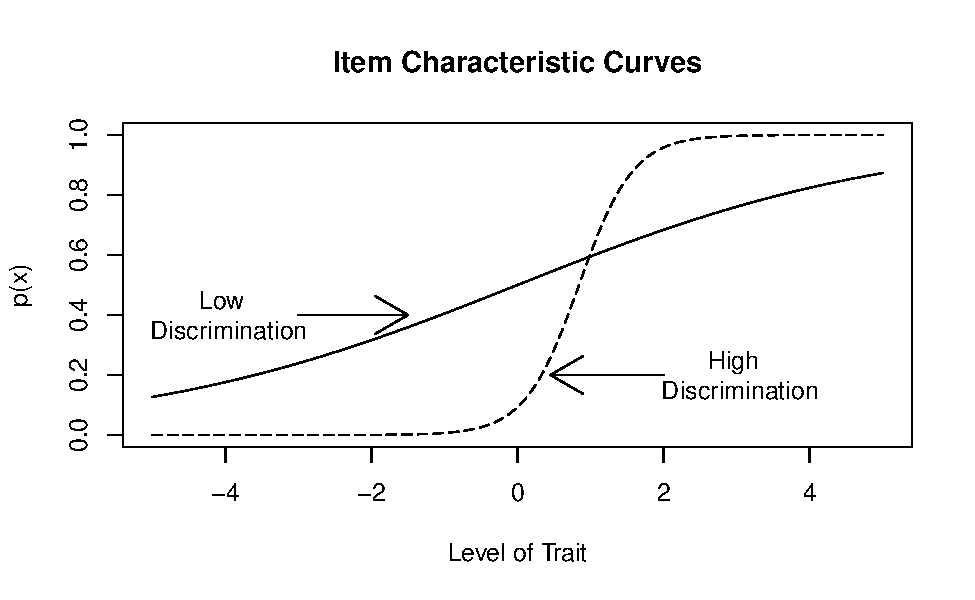
\includegraphics{ICC_project_files/figure-latex/unnamed-chunk-1-1.pdf}
\caption{\label{fig:unnamed-chunk-1}Item characteristic curves primarily reflecting differences in discrimination.}
\end{figure}

Assessment specialists who examine ICCs usually do so from within the psychometric framework of either Item Response Theory or Rasch modeling. These frameworks provide the parameters necessary to plot the curves. Rasch models only estimate difficulty, and assume that differences in discrimination represent flaws in measurement. The IRT 2 parameter logistic model (2PL), however, models both item difficulty as well as item discrimination. Item difficulty (the \emph{b}-parameter) is scaled as the trait level associated with a 50\% likelihood of correct response (e.g., it is scaled to \(\theta\)). Item discrimination (\emph{a}-parameter) is the degree to which an item differentiates across individuals who are characterized as being relatively lower or higher on the trait. From a Classical Test Theory (CTT) orientation, item difficulty is most commonly represented by the percent of individuals answering the item correctly (also referred to as a \emph{p-value}). Item discrimination can be conveyed via a few CTT indices, but the most commonly calculated and consulted index is the corrected item total correlation.

Assessment specialists who consult these CTT parameters don't typically (to our knowledge!) attempt to represent them visually, as is common in IRT and Rasch applications. However, there is perhaps little opposition for them not to do so, as ICCs based on CTT parameters could provide snapshot psychometric information as valuable as those gained from IRT- or Rasch-derived ICCs. The largest obstacle to psychometricians regarding CTT-derived visuals is likely the concept of invariance, which refers to IRT parameter independence across item and person estimates. However, this property is often overstated, as invariance is only attained with perfect model-data fit (which never occurs), and is also only true after being subjected to linear transformation (commonly across samples). Additionally, several comparative investigations have noted commonality between IRT and CTT difficulty and discrimination estimates as well as relative stability of CTT estimates when samples are large and/or judisciously constructed (Fan, 1998). Fan in fact summarizes that the IRT and CTT frameworks ``\ldots produce very similar item and person statistics'' (p.379). Hambleton and Jones (1993) concluded that ``no study provides enough empirical evidence on the extent of disparity between the two frameworks and the superiority of IRT over CTT despite the theoretical differences.''

Fan (1998) looked at the correlations between ability estimates and item difficulty in CTT and all three IRT models. These correlations were very high, generally between .80 and .90. As for item discrimination, correlations were moderate to high, with only a few being very low.\footnote{\ldots and in fact, as is presented below, the relationship between the IRT and CTT discrimination indices is non-linear - the correlation is an inappropriate index to capture the magnitude of this relationship.}

Fan (1998) also investigated item invariance for all models. In theory, the major advantage of IRT models over CTT is that the latter has an interdependency between the item and person statistics, whereas IRT has no such dependency. For example, within CTT examinations, the average item difficulty is equivalent to the average person score - these indices are merely reflective of averages computed across rows or columns.

What Fan (1998) found in his study, however, did not support the purported invariant advantage of IRT parameters over CTT indices. Both CTT item difficulty and discrimination degrees of invariance were highly correlated with those of IRT, indicating that they were highly comparable.

\begin{quote}
\begin{quote}
NEED MORE - GRAB FROM OLD PAPER OR FIND NEW COMPARATIVE STUDIES
\end{quote}
\end{quote}

\hypertarget{relationship-between-irt-and-ctt-indices}{%
\subsection{Relationship between IRT and CTT indices}\label{relationship-between-irt-and-ctt-indices}}

Lord (2012) described a function that approximates the relationship between IRT parameters and the CTT discrimination index of an item-test biserial correlation:

\[a_i\cong \frac{r_i}{\sqrt{1-r_i^2}}\]

This formula wasn't intended for practical purposes but rather to assist in the conceptual comprehension of the discrimination parameter in IRT for people who were more familiar with CTT procedures. In an effort to move from the conceptual to a practical application, Kulas et al. (2017) proposed a modification that minimized the average residual (either \(a_i\) or \(r_i\), where \(r_i\) is the \emph{corrected} item-total \emph{point-biserial} correlation).

The Kulas et al. (2017) investigations (both simulated and utilizing real-world test data) identified systematic predictive differences across items with differing item difficulty values, so their recommended formula included a specification for item difficulty. This revised formula is used in the current presentation:

\[\hat{a_i}\cong[(.51 + .02z_g + .3z_g^2)r]+[(.57 - .009z_g + .19z_g^2)\frac{e^r-e^{-r}}{e-e^r}]\]

Where \(g\) is the absolute deviation from 50\% responding an item correctly and 50\% responding incorrectly (e.g., a ``p-value'' of .5). \(Z_g\) is the standard normal deviate associated with \(g\). The transformation of the standard p-value was recommended in order to scale this index along an interval-level metric more directly anaologous to the IRT \emph{b} parameter. Figure XX visualizes the re-specifications of Lord's formula at p-values (difficulty) of .5, .3 (or .7), and .1 (or .9) and highlights the nonlinear nature of this relationship - especially so at high levels of discrimination.

\begin{figure}
\centering
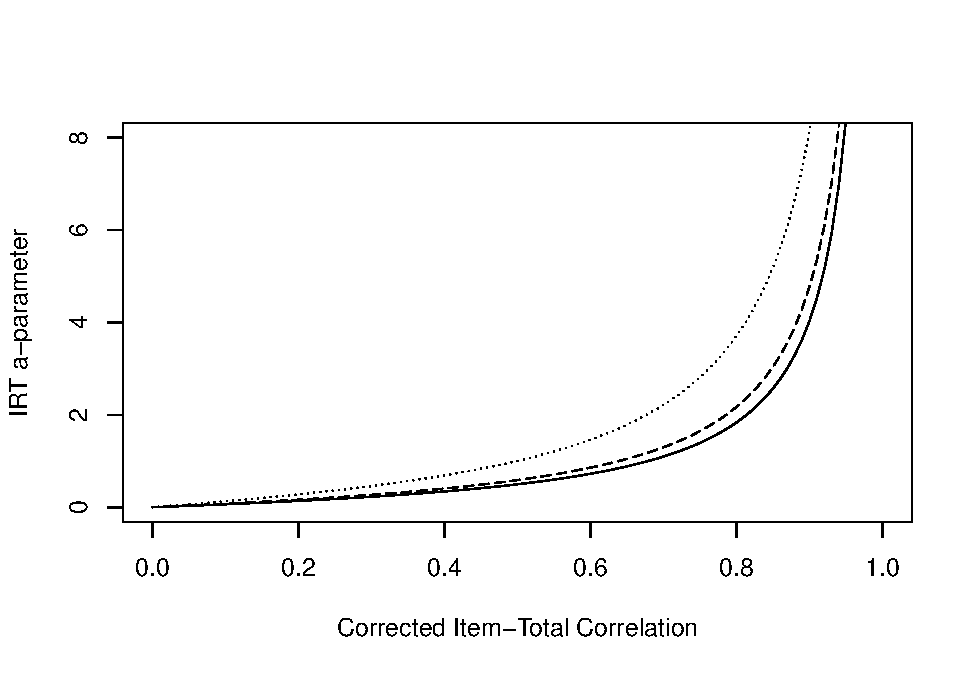
\includegraphics{ICC_project_files/figure-latex/acorrected-1.pdf}
\caption{\label{fig:acorrected}Empricially-derived functional relationship between the IRT \emph{a} parameter and the CTT corrected-item total correlation as a function of item difficulty (p-value; solid = .5, dashed = .3/.7, dotted = .1/.9).}
\end{figure}

As we can see, the higher the corrected item-total correlations, the higher the estimated IRT a-parameter (discrimination). Also, as the p-values (difficulty) deviates from 0, the relationship between the estimated IRT a-parameter and the corrected item-total correlations becomes stronger.

Practitioners and researchers that don't use IRT or Rasch models and instead opt to follow a CTT philosophy would benefit from having ICCs that use CTT statistics. This study intends to show evidence of the overlapping nature of CTT and IRT parameters when it comes to plotting ICCs.

\hypertarget{study-1---estimating-ctt-derived-iccs}{%
\section{Study 1 - Estimating CTT-Derived ICCs}\label{study-1---estimating-ctt-derived-iccs}}

The purpose of study 1 is to look at the visualizations resulting from Kulas et al. (2017) formula on simulated data. We hypothesize that the relationship between the estimated IRT a-parameter and the corrected item-total correlations will be stronger as the later deviates from 0, which would mean that the item has more discrimination.

\hypertarget{procedure-and-methods}{%
\subsection{Procedure and methods}\label{procedure-and-methods}}

We simulated data using Han (2007) software. Our sample was 10,000 observations, with a mean of 0 and a standard deviation of 1. The number of items were 100, with response categories of either correct or incorrect (1 and 0).The mean for the a parameter was 2, and the standard deviation 0.8. The mean for parameter b was 0 and the standard deviation 0.5.

\hypertarget{results}{%
\subsection{Results}\label{results}}

\hypertarget{study-2---evaluating-the-comparability-of-irt-and-ctt-iccs}{%
\section{Study 2 - Evaluating the Comparability of IRT and CTT ICCs}\label{study-2---evaluating-the-comparability-of-irt-and-ctt-iccs}}

The purpose of study 2 is to simulates a lot of test data and then generate ICCs based on the IRT model and then we compare that to our CTT estimates.

\hypertarget{procedure-and-materials}{%
\subsection{Procedure and materials}\label{procedure-and-materials}}

The same simulated data as in study 1 was used. The mirt package was used to compute the IRT statistics. The blue curves were plotted using 2PL IRT parameters (a and b), while the red curves were plotted using CTT parameters (p-values and corrected item-total correlations, modifying them with Kulas et al. (2017) formulas).

\hypertarget{results-1}{%
\subsection{Results}\label{results-1}}

We used R {[}Version 4.1.1; R Core Team (2020){]} and the R-packages \emph{\}ape} {[}@\}R-ape{]}, \emph{dplyr} {[}Version 1.0.7; Wickham et al. (2021){]}, \emph{DT} {[}Version 0.19; Xie et al. (2021){]}, \emph{forcats} {[}Version 0.5.1; Wickham (2021a){]}, \emph{formattable} (Ren \& Russell, 2021), \emph{geiger} {[}Version 2.0.7; Alfaro et al. (2009); Eastman et al. (2011); Slater et al. (2012); Harmon et al. (2008); Pennell et al. (2014){]}, \emph{ggplot2} {[}Version 3.3.5; Wickham (2016){]}, \emph{gridExtra} {[}Version 2.3; Auguie (2017){]}, \emph{irtplay} {[}Version 1.6.2; Lim (2020){]}, \emph{jpeg} {[}Version 0.1.9; Urbanek (2021){]}, \emph{knitr} {[}Version 1.34; Xie (2015){]}, \emph{lattice} {[}Version 0.20.44; Sarkar (2008); Sarkar and Andrews (2019){]}, \emph{latticeExtra} {[}Version 0.6.29; Sarkar and Andrews (2019){]}, \emph{markdown} {[}Version 1.1; Allaire et al. (2019); Xie et al. (2018); Xie et al. (2020){]}, \emph{mirt} {[}Version 1.34; Chalmers (2012){]}, \emph{officer} (Gohel, 2021), \emph{papaja} {[}Version 0.1.0.9997; Aust and Barth (2020){]}, \emph{pdftools} {[}Version 3.0.1; Ooms (2021){]}, \emph{psych} {[}Version 2.1.9; Revelle (2021){]}, \emph{purrr} {[}Version 0.3.4; Henry and Wickham (2020){]}, \emph{readr} {[}Version 2.0.1; Wickham and Hester (2021){]}, \emph{readxl} {[}Version 1.3.1; Wickham and Bryan (2019){]}, \emph{reticulate} {[}Version 1.22; Ushey et al. (2021){]}, \emph{rmarkdown} {[}Version 2.11; Xie et al. (2018); Xie et al. (2020){]}, \emph{shiny} {[}Version 1.7.0; Chang et al. (2021){]}, \emph{stringr} {[}Version 1.4.0; Wickham (2019){]}, \emph{tibble} {[}Version 3.1.4; Müller and Wickham (2021){]}, \emph{tidyr} {[}Version 1.1.3; Wickham (2021b){]}, \emph{tidyverse} {[}Version 1.3.1; Wickham et al. (2019){]}, and \emph{tinytex} {[}Version 0.33; Xie (2019){]} for all our analyses. The area between ICC's was calculated between CTT-derived and IRT-derived ICCs. The average difference for all 100 curves was 0.35.

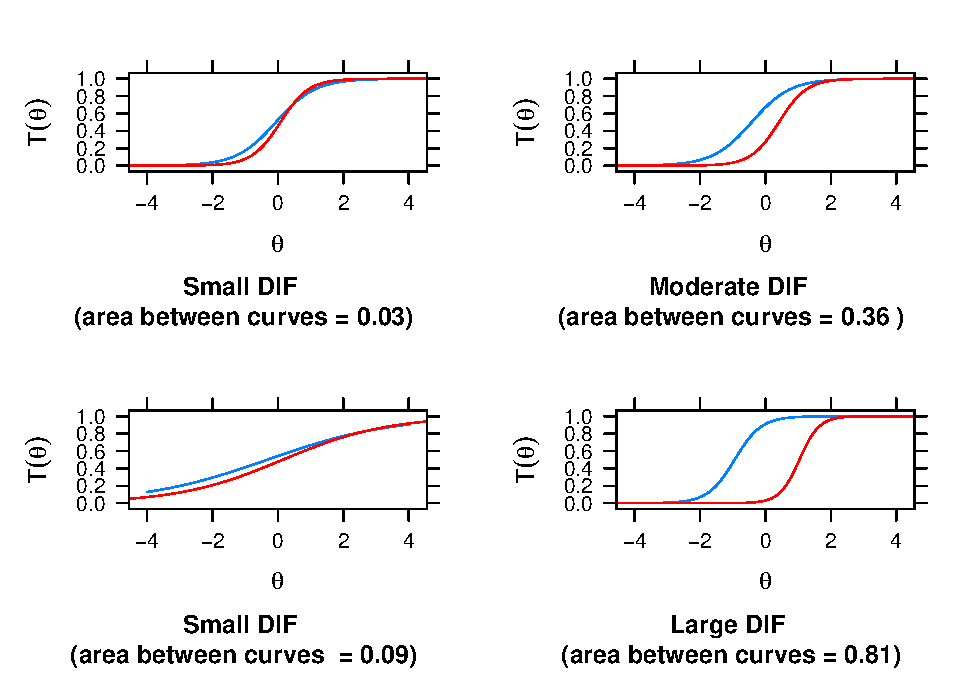
\includegraphics{ICC_project_files/figure-latex/plotting-1.pdf}

\begin{figure}
\centering
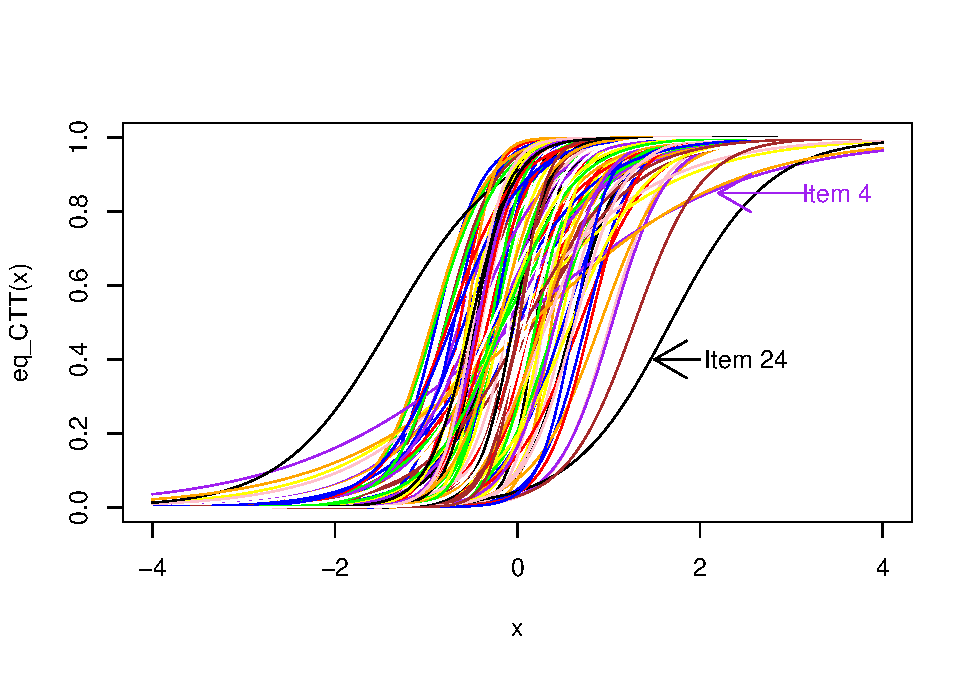
\includegraphics{ICC_project_files/figure-latex/AUC-1.pdf}
\caption{\label{fig:AUC}ICCs derived from only CTT parameters (with two noteworthy ICCs annotated).}
\end{figure}

\begin{figure}
\centering
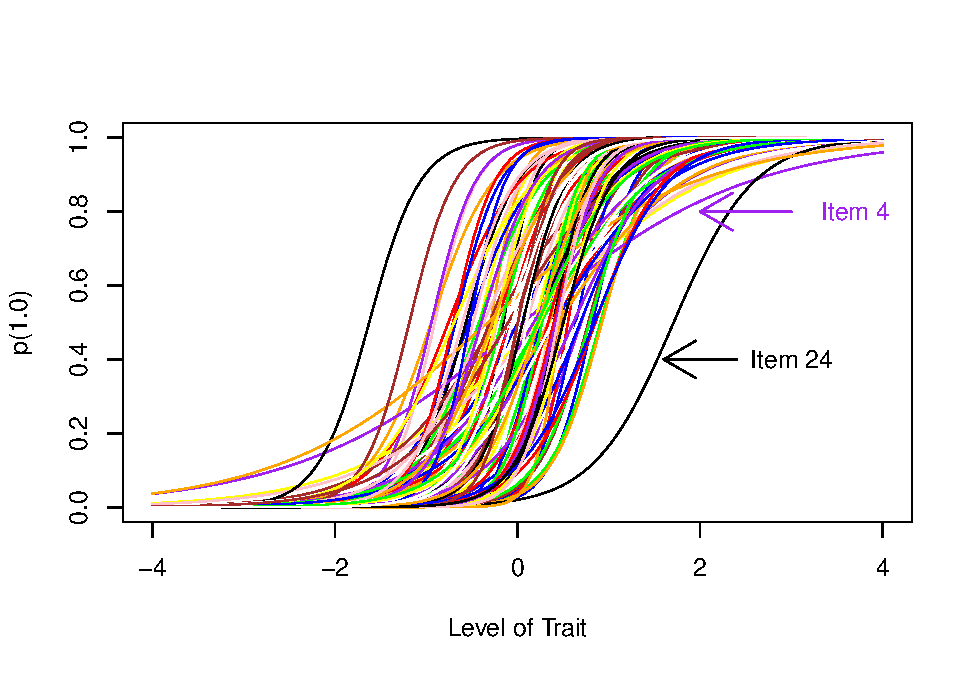
\includegraphics{ICC_project_files/figure-latex/irtcurves-1.pdf}
\caption{\label{fig:irtcurves}Typical ICCs derived from IRT parameters (same noteworthy items annotated).}
\end{figure}

\hypertarget{results-2}{%
\section{Results}\label{results-2}}

\hypertarget{discussion}{%
\section{Discussion}\label{discussion}}

If this general idea is well-recieved (SIOP members would seem to represent a great barometer!) we would like to stress the CTT ICCs via further and more extensive conditions. That is, are there patterns that help explain CTT ICCs that diverge from their IRT counterparts? Although our simulations did generate a range of item difficulties and discriminations, we have not yet fully explored systematic patterns of extremly difficult/easy items as well as very poorly discriminating items. If patterns emerge, we would like to model predicted discrepancies via incorporating error bars within our visualizations.

Additionally, if there is interest in this general idea we would likely publish our function as a small \texttt{R} package, perhaps to supplement the \texttt{psych} package's ``alpha'' function, which produces corrected item-total correlations as well as p-values within the same output table (e.g., the ``input'' data is already available in tabular format).

\newpage

\hypertarget{references}{%
\section{References}\label{references}}

\begingroup
\setlength{\parindent}{-0.5in}
\setlength{\leftskip}{0.5in}

\hypertarget{refs}{}
\begin{CSLReferences}{1}{0}
\leavevmode\hypertarget{ref-R-geiger_a}{}%
Alfaro, M., Santini, F., Brock, C., Alamillo, H., Dornburg, A., Rabosky, D., Carnevale, G., \& Harmon, L. (2009). Nine exceptional radiations plus high turnover explain species diversity in jawed vertebrates. \emph{Proceedings of the National Academy of Sciences of the United States of America}, \emph{106}, 13410--13414.

\leavevmode\hypertarget{ref-R-markdown}{}%
Allaire, J., Horner, J., Xie, Y., Marti, V., \& Porte, N. (2019). \emph{Markdown: Render markdown with the c library 'sundown'}. \url{https://CRAN.R-project.org/package=markdown}

\leavevmode\hypertarget{ref-R-gridExtra}{}%
Auguie, B. (2017). \emph{gridExtra: Miscellaneous functions for "grid" graphics}. \url{https://CRAN.R-project.org/package=gridExtra}

\leavevmode\hypertarget{ref-R-papaja}{}%
Aust, F., \& Barth, M. (2020). \emph{{papaja}: {Create} {APA} manuscripts with {R Markdown}}. \url{https://github.com/crsh/papaja}

\leavevmode\hypertarget{ref-R-mirt}{}%
Chalmers, R. P. (2012). {mirt}: A multidimensional item response theory package for the {R} environment. \emph{Journal of Statistical Software}, \emph{48}(6), 1--29. \url{https://doi.org/10.18637/jss.v048.i06}

\leavevmode\hypertarget{ref-R-shiny}{}%
Chang, W., Cheng, J., Allaire, J., Sievert, C., Schloerke, B., Xie, Y., Allen, J., McPherson, J., Dipert, A., \& Borges, B. (2021). \emph{Shiny: Web application framework for r}. \url{https://CRAN.R-project.org/package=shiny}

\leavevmode\hypertarget{ref-R-geiger_b}{}%
Eastman, J., Alfaro, M., Joyce, P., Hipp, A., \& Harmon, L. (2011). A novel comparative method for identifying shifts in the rate of character evolution on trees. \emph{Evolution}, \emph{65}, 3578--3589.

\leavevmode\hypertarget{ref-fan1998item}{}%
Fan, X. (1998). Item response theory and classical test theory: An empirical comparison of their item/person statistics. \emph{Educational and Psychological Measurement}, \emph{58}(3), 357--381.

\leavevmode\hypertarget{ref-R-officer}{}%
Gohel, D. (2021). \emph{Officer: Manipulation of microsoft word and PowerPoint documents}. \url{https://CRAN.R-project.org/package=officer}

\leavevmode\hypertarget{ref-hambleton1993comparison}{}%
Hambleton, R. K., \& Jones, R. W. (1993). Comparison of classical test theory and item response theory and their applications to test development. \emph{Educational Measurement: Issues and Practice}, \emph{12}(3), 38--47.

\leavevmode\hypertarget{ref-han2007wingen3}{}%
Han, K. (2007). WinGen3: Windows software that generates IRT parameters and item responses {[}computer program{]}. \emph{Amherst, MA: Center for Educational Assessment, University of Massachusetts Amherst}.

\leavevmode\hypertarget{ref-R-geiger_d}{}%
Harmon, L., Weir, J., Brock, C., Glor, R., \& Challenger, W. (2008). GEIGER: Investigating evolutionary radiations. \emph{Bioinformatics}, \emph{24}, 129--131.

\leavevmode\hypertarget{ref-R-purrr}{}%
Henry, L., \& Wickham, H. (2020). \emph{Purrr: Functional programming tools}. \url{https://CRAN.R-project.org/package=purrr}

\leavevmode\hypertarget{ref-kulas2017approximate}{}%
Kulas, J. T., Smith, J. A., \& Xu, H. (2017). Approximate functional relationship between IRT and CTT item discrimination indices: A simulation, validation, and practical extension of lord's (1980) formula. \emph{Journal of Applied Measurement}, \emph{18}(4), 393--407.

\leavevmode\hypertarget{ref-R-irtplay}{}%
Lim, H. (2020). \emph{Irtplay: Unidimensional item response theory modeling}. \url{https://CRAN.R-project.org/package=irtplay}

\leavevmode\hypertarget{ref-lord2012applications}{}%
Lord, F. M. (2012). \emph{Applications of item response theory to practical testing problems}. Routledge.

\leavevmode\hypertarget{ref-R-tibble}{}%
Müller, K., \& Wickham, H. (2021). \emph{Tibble: Simple data frames}. \url{https://CRAN.R-project.org/package=tibble}

\leavevmode\hypertarget{ref-R-pdftools}{}%
Ooms, J. (2021). \emph{Pdftools: Text extraction, rendering and converting of PDF documents}. \url{https://CRAN.R-project.org/package=pdftools}

\leavevmode\hypertarget{ref-R-geiger_e}{}%
Pennell, M., Eastman, J., Slater, G., Brown, J., Uyeda, J., Fitzjohn, R., Alfaro, M., \& Harmon, L. (2014). Geiger v2.0: An expanded suite of methods for fitting macroevolutionary models to phylogenetic trees. \emph{Bioinformatics}, \emph{30}, 2216--2218.

\leavevmode\hypertarget{ref-R-base}{}%
R Core Team. (2020). \emph{R: A language and environment for statistical computing}. R Foundation for Statistical Computing. \url{https://www.R-project.org/}

\leavevmode\hypertarget{ref-R-formattable}{}%
Ren, K., \& Russell, K. (2021). \emph{Formattable: Create 'formattable' data structures}. \url{https://CRAN.R-project.org/package=formattable}

\leavevmode\hypertarget{ref-R-psych}{}%
Revelle, W. (2021). \emph{Psych: Procedures for psychological, psychometric, and personality research}. Northwestern University. \url{https://CRAN.R-project.org/package=psych}

\leavevmode\hypertarget{ref-R-lattice}{}%
Sarkar, D. (2008). \emph{Lattice: Multivariate data visualization with r}. Springer. \url{http://lmdvr.r-forge.r-project.org}

\leavevmode\hypertarget{ref-R-latticeExtra}{}%
Sarkar, D., \& Andrews, F. (2019). \emph{latticeExtra: Extra graphical utilities based on lattice}. \url{https://CRAN.R-project.org/package=latticeExtra}

\leavevmode\hypertarget{ref-R-geiger_c}{}%
Slater, G., Harmon, L., Wegmann, D., Joyce, P., Revell, L., \& Alfaro, M. (2012). Fitting models of continuous trait evolution to incompletely sampled comparative data using approximate bayesian computation. \emph{Evolution}, \emph{66}, 752--762.

\leavevmode\hypertarget{ref-R-jpeg}{}%
Urbanek, S. (2021). \emph{Jpeg: Read and write JPEG images}. \url{https://CRAN.R-project.org/package=jpeg}

\leavevmode\hypertarget{ref-R-reticulate}{}%
Ushey, K., Allaire, J., \& Tang, Y. (2021). \emph{Reticulate: Interface to 'python'}. \url{https://CRAN.R-project.org/package=reticulate}

\leavevmode\hypertarget{ref-R-ggplot2}{}%
Wickham, H. (2016). \emph{ggplot2: Elegant graphics for data analysis}. Springer-Verlag New York. \url{https://ggplot2.tidyverse.org}

\leavevmode\hypertarget{ref-R-stringr}{}%
Wickham, H. (2019). \emph{Stringr: Simple, consistent wrappers for common string operations}. \url{https://CRAN.R-project.org/package=stringr}

\leavevmode\hypertarget{ref-R-forcats}{}%
Wickham, H. (2021a). \emph{Forcats: Tools for working with categorical variables (factors)}. \url{https://CRAN.R-project.org/package=forcats}

\leavevmode\hypertarget{ref-R-tidyr}{}%
Wickham, H. (2021b). \emph{Tidyr: Tidy messy data}. \url{https://CRAN.R-project.org/package=tidyr}

\leavevmode\hypertarget{ref-R-tidyverse}{}%
Wickham, H., Averick, M., Bryan, J., Chang, W., McGowan, L. D., François, R., Grolemund, G., Hayes, A., Henry, L., Hester, J., Kuhn, M., Pedersen, T. L., Miller, E., Bache, S. M., Müller, K., Ooms, J., Robinson, D., Seidel, D. P., Spinu, V., \ldots{} Yutani, H. (2019). Welcome to the {tidyverse}. \emph{Journal of Open Source Software}, \emph{4}(43), 1686. \url{https://doi.org/10.21105/joss.01686}

\leavevmode\hypertarget{ref-R-readxl}{}%
Wickham, H., \& Bryan, J. (2019). \emph{Readxl: Read excel files}. \url{https://CRAN.R-project.org/package=readxl}

\leavevmode\hypertarget{ref-R-dplyr}{}%
Wickham, H., François, R., Henry, L., \& Müller, K. (2021). \emph{Dplyr: A grammar of data manipulation}. \url{https://CRAN.R-project.org/package=dplyr}

\leavevmode\hypertarget{ref-R-readr}{}%
Wickham, H., \& Hester, J. (2021). \emph{Readr: Read rectangular text data}. \url{https://CRAN.R-project.org/package=readr}

\leavevmode\hypertarget{ref-R-knitr}{}%
Xie, Y. (2015). \emph{Dynamic documents with {R} and knitr} (2nd ed.). Chapman; Hall/CRC. \url{https://yihui.org/knitr/}

\leavevmode\hypertarget{ref-R-tinytex}{}%
Xie, Y. (2019). TinyTeX: A lightweight, cross-platform, and easy-to-maintain LaTeX distribution based on TeX live. \emph{TUGboat}, \emph{1}, 30--32. \url{http://tug.org/TUGboat/Contents/contents40-1.html}

\leavevmode\hypertarget{ref-R-rmarkdown_a}{}%
Xie, Y., Allaire, J. J., \& Grolemund, G. (2018). \emph{R markdown: The definitive guide}. Chapman; Hall/CRC. \url{https://bookdown.org/yihui/rmarkdown}

\leavevmode\hypertarget{ref-R-DT}{}%
Xie, Y., Cheng, J., \& Tan, X. (2021). \emph{DT: A wrapper of the JavaScript library 'DataTables'}. \url{https://CRAN.R-project.org/package=DT}

\leavevmode\hypertarget{ref-R-rmarkdown_b}{}%
Xie, Y., Dervieux, C., \& Riederer, E. (2020). \emph{R markdown cookbook}. Chapman; Hall/CRC. \url{https://bookdown.org/yihui/rmarkdown-cookbook}

\end{CSLReferences}

\endgroup


\end{document}
